\chapter{MPI}

\section{Introduction}

The \textbf{Message Passing Interface (MPI)} is a standardized library that implements the distributed memory programming model. Its primary purpose is to facilitate data movement between distinct address spaces in a parallel computing environment.

In MPI, each process operates as an \textbf{independent} entity with its own private memory space. From a programming perspective, memory management within each process follows the same principles as sequential programming, making it conceptually straightforward for developers.

Processes interact through explicit message passing for both synchronization and data exchange. This communication model requires \textbf{explicit collaboration} between processes - data is only shared when processes explicitly send and receive messages.

It's important to note that MPI is implemented as a \textbf{library} rather than a programming language. This means that all parallel operations are performed through library function calls, which provides flexibility in terms of language integration while maintaining a consistent interface across different platforms.

So how is MPI structured? It is organized into several key components:

\begin{itemize}
    \item the message to send
    \item the length of the message
    \item the receiver process
    \item the framework this message belongs to
\end{itemize}

\begin{codeblock}[language=C]
int MPI_Send(
    const void *buf,        /* starting address of send buffer */
    int count,              /* number of elements in send buffer */
    MPI_Datatype datatype,  /* datatype of each buffer element */
    int dest,               /* rank of destination */
    int tag,                /* message tag */
    MPI_Comm comm           /* communicator */
)
\end{codeblock}

we'll see it more in detail later. In the same way, there must be a way to receive a message from another process; this method should accept the following parameters:
\begin{itemize}
    \item where to store the message
    \item the length of the message
    \item the sender process
    \item the framework this message belongs to
\end{itemize}

\begin{codeblock}[language=C]
int MPI_Recv(
    void *buf,              /* starting address of receive buffer */
    int count,              /* number of elements in receive buffer */
    MPI_Datatype datatype,  /* datatype of each buffer element */
    int source,             /* rank of source */
    int tag,                /* message tag */
    MPI_Comm comm,          /* communicator */
    MPI_Status *status      /* status object */
)
\end{codeblock}

So, we expect that there must be point-to-point
\begin{itemize}
    \item a way to send messages
    \item a corresponding way to receive messages
    \item a way to know “the names” in “the framework”
\end{itemize}

Since sometimes we need to broadcast messages, it would be nice if:
\begin{itemize}
    \item there was a \textbf{broadcasting} (one-to-many) mechanism
    \item there was a \textbf{collection} mechanism (many-to-one) mechanism
    \item the answer/collection was possible \textbf{many-to-many}
\end{itemize}

Let's create the first and most basic MPI program.

\begin{codeblock}[language=C]
#include <mpi.h>
int main( int argc, char **argv ) {
    MPI_Init( &argc, &argv ); /* Initialize MPI */

    MPI_Finalize( ); /* Terminate MPI */
    return 0; /* explicitly return as best practice */
}
\end{codeblock}

The second most simple MPI program is obviously "hello MPI world"!
\begin{codeblock}[language=C]
#include <mpi.h>

int main( int argc, char **argv ) {
    int Myrank, Nprocs;

    MPI_Init( &argc, &argv ); /* Initialize MPI */

    MPI_Comm_rank( MPI_COMM_WORLD, &Myrank ); /* Get my rank */
    MPI_Comm_size( MPI_COMM_WORLD, &Nprocs ); /* Get number of processes */

    printf( "Hello from process %d of %d\n", Myrank, Nprocs );

    MPI_Finalize( ); /* Terminate MPI */
    return 0; /* explicitly return as best practice */
}
\end{codeblock}

\begin{tipsblock}[The man page]
    There exist a wonderful thing, invented by smart people, called \textbf{man page}. It is a documentation of the functions provided by the system and by libraries.
    To access it you can use the command
    \begin{codeblock}[language=bash]
        man MPI_$FUNCTION$
    \end{codeblock}
    where \texttt{\$FUNCTION\$} is the name of the function you want to know more about.
\end{tipsblock}

\subsection*{Communicators}

Communicators and groups are a very central concepts in MPI: tasks can form groups (a task can belong to more than one group) and the same group can be in different situations.

The \bfit{communicator} is the combination of a group and its “context”.

\begin{figure}[H]
    \centering
    \includegraphics[width=\textwidth]{assets/mpi1.png}
    \caption{Communicator and groups}
    \label{fig:communicator}
\end{figure}

You can build as many groups as you want, and they may or not have a communicator. However, if you want to communicate among tasks in a group, you need a communicator.
This functionality offers the capability of isolating communication between application modules with an effective “sandbox” for different contexts.
For instance, a parallel library and your application will use internally their own communicator, separating contexts.

By creating groups of MPI processes, that may or not overlap with each other, it is possible to
\begin{itemize}
    \item separate contexts within different modules of the same application
    (useful or even advisable)
    \item express multiple levels of parallelism
\end{itemize}

MPI provides several predefined communicators that are available after initialization:

\begin{itemize}
    \item \texttt{MPI\_COMM\_WORLD} is the default communicator available right after the call to \texttt{MPI\_Init}. Its group contains all the tasks started by your job.
    
    \item \texttt{MPI\_COMM\_NULL} signals an invalid or non-existent communicator. This is often used as a return value to indicate errors in communicator operations.
    
    \item \texttt{MPI\_COMM\_SELF} contains only the process itself. This is useful when a process needs to communicate with itself.
    
    \item \texttt{MPI\_GROUP\_NULL} signals an invalid or non-existent group. Similar to \texttt{MPI\_COMM\_NULL}, it's used to indicate errors in group operations.
\end{itemize}

These predefined communicators serve as fundamental building blocks for MPI communication patterns and are essential for both basic and advanced MPI programming.

\begin{observationblock}
    Always create a separated \textbf{context} for the application you're writing.
    \begin{codeblock}[language=C]
#include <mpi.h>

int main(int argc, char **argv) {
    int Myranlk, Ntasks;
    int mpi_provided_thread_level;
    MPI_Comm myCOMM_WORLD;

    MPI_Init_thread(&argc, &argv, MPI_THREAD_SINGLE, &mpi_provided_thread_level);
    MPI_Comm_dup(MPI_COMM_WORLD, &myCOMM_WORLD); /* create a separated context */

    MPI_Comm_size(&Ntasks, myCOMM_WORLD);
    MPI_Comm_rank(&Myranlk, myCOMM_WORLD);
    ... 
}
    \end{codeblock}
\end{observationblock}

\section{Point-to-point communications}

\subsection*{Building blocks: Send and Receive}

Recalling the previous section, MPI provides two basic functions for sending and receiving messages between processes:

\begin{codeblock}[language=C]
int MPI_Send(
    const void *buf,        /* starting address of send buffer */
    int count,              /* number of elements in send buffer */
    MPI_Datatype datatype,  /* datatype of each buffer element */
    int dest,               /* rank of destination */
    int tag,                /* message tag */
    MPI_Comm comm           /* communicator */
)
\end{codeblock}

\begin{codeblock}[language=C]
int MPI_Recv(
    void *buf,              /* starting address of receive buffer */
    int count,              /* number of elements in receive buffer */
    MPI_Datatype datatype,  /* datatype of each buffer element */
    int source,             /* rank of source */
    int tag,                /* message tag */
    MPI_Comm comm,          /* communicator */
    MPI_Status *status      /* status object */
)
\end{codeblock}

We can say that the message consists of a \textbf{body} (\texttt{buf}, \texttt{count}, \texttt{datatype}) and an \textbf{envelop} (\texttt{dest}, \texttt{tag}, \texttt{comm}).
The data type is a fundamental concept in MPI. It defines the type of data being sent or received. MPI provides a variety of predefined data types, including:

\begin{table}[H]
    \centering
    \begin{tabular}{|l|l|}
        \hline
        \textbf{MPI DataType} & \textbf{C DataType} \\
        \hline
        \plaintt{MPI\_CHAR} & \plaintt{char} \\
        \plaintt{MPI\_BYTE} & \plaintt{unsigned char} \\
        \plaintt{MPI\_SHORT}, \plaintt{MPI\_UNSIGNED\_SHORT} & (\plaintt{unsigned}) \plaintt{short int} \\
        \plaintt{MPI\_INT}, \plaintt{MPI\_UNSIGNED\_INT} & (\plaintt{unsigned}) \plaintt{int} \\
        \plaintt{MPI\_LONG}, \plaintt{MPI\_UNSIGNED\_LONG} & (\plaintt{unsigned}) \plaintt{long int} \\
        \plaintt{MPI\_LONG\_LONG}, \plaintt{MPI\_UNSIGNED\_LONG\_LONG} & (\plaintt{unsigned}) \plaintt{long long int} \\
        \plaintt{MPI\_FLOAT} & \plaintt{float} \\
        \plaintt{MPI\_DOUBLE} & \plaintt{double} \\
        \plaintt{MPI\_LONG\_DOUBLE} & \plaintt{long double} \\
        \plaintt{MPI\_PACKED} & \plaintt{--} \\
        \hline
    \end{tabular}
    \caption{Correspondence between MPI predefined datatypes and C datatypes.}
    \label{tab:mpi-c-datatypes}
\end{table}

\begin{exampleblock}[Send and Receive Example]
    \begin{codeblock}[language=C]
int N;
if ( Myrank == 0 )
    MPI_Send( &N, 1, MPI_INT, 1, 0, MPI_COMM_WORLD );
else if ( Myrank == 1 ) {
    MPI_Status status;
    MPI_Recv( &N, 1, MPI_INT, 0, 0, MPI_COMM_WORLD, &status );
}
else if ( Myrank == 1 )
    MPI_Recv( &N, 1, MPI_INT, 0, 0, MPI_COMM_WORLD, MPI_STATUS_IGNORE );
    \end{codeblock}

    \underline{\textbf{NOTE}}: \plaintt{MPI\_STATUS\_IGNORE} is always valid instead of putting an \plaintt{MPI\_Status} varible's address as last argument of \plaintt{MPI\_Recv}
\end{exampleblock}

\begin{exampleblock}[Sending things of different types]
    \begin{codeblock}[language=C]
typedef struct {
    int i, j;
    double d, f;
    char s[4];
} my_data;

unsigned int length = N * sizeof(my_data);

if (Myrank == 0) {
    MPI_Send(data, length, MPI_BYTE, 1, 0, MPI_COMM_WORLD);
} else if (Myrank == 1) {
    MPI_Recv(data, length, MPI_BYTE, 0, 0, MPI_COMM_WORLD,
             MPI_STATUS_IGNORE);
}
    \end{codeblock}
\end{exampleblock}

Why the \texttt{MPI\_STATUS} in \texttt{MPI\_Recv}?

\begin{itemize}
    \item The \texttt{MPI\_Recv}'s argument count provides the maximum number of elements that the call expects to receive. If the message exceeds that count, an error is thrown. Hence, you don't know whether \texttt{MPI\_Recv} has got $n\leq count$ elements. 
    \item Valid values for the source and tag arguments are \texttt{MPI\_ANY\_SOURCE} and \texttt{MPI\_ANY\_TAG}, so that the task could receive messages from anybody with any tag.
    \item However, it may be that, once received, you need to know who was the sender, which was the tag and what is the size of the received message. Use \texttt{status.TAG, status.MPI\_SOURCE} and \texttt{MPI\_Get\_count(\&status, MPI\_type\_used, \&count)} to get this information.
\end{itemize}

You may also want to know whether a message is arriving, from who and how large before to actually get it. 

\begin{codeblock}[language=C]
MPI_Status status;

// Probe for an incoming message from whatever process and whatever tag
MPI_Probe(MPI_ANY_SOURCE, MPI_ANY_TAG, MPI_COMM_WORLD, &status);

source = status.MPI_SOURCE; // Get the source
tag = status.MPI_TAG;       // Get the tag
MPI_Get_count(&status, MPI_BYTE, &number_amount); // Get the size
char *buffer = (char *)malloc(number_amount); // Allocate the buffer
MPI_Recv(buffer, number_amount, MPI_BYTE, source, tag, MPI_COMM_WORLD, &status); // Now receive the message
... 
// Probe for an incoming message from process zero with a precise tag 
MPI_Probe(0, 123, MPI_COMM_WORLD, &status);
... 
\end{codeblock}

\begin{observationblock}[Safety first]
    How can we be sure that the communication has ended and the data have all been received?

    The MPI standard prescribes that \texttt{MPI\_Send} returns when it is safe to modify the send buffer. So, whenever \texttt{MPI\_Send} returns, it is safe to act on the memory region that has been sent. However, as a more general discussion, there are two main protocols:
    \begin{enumerate}
        \item \textbf{Eager protocol}
        
        \begin{minipage}{0.48\textwidth}
            Here, \texttt{MPI\_Send} returns before the data actually reach the destination. More correctly, it returns without knowing whether that happened already or not. The MPI library copies the sent data on local buffer, either on the sender size or the receiver size. The actual transfer will complete afterwards and the \texttt{MPI\_Send} returns. 

            This protocol is used for \textbf{small messages} usually. 
        \end{minipage}
        \begin{minipage}{0.48\textwidth}
            \begin{figure}[H]
                \centering
                \includegraphics[width=0.6\textwidth]{assets/mpi2.png}
                \caption{Eager protocol}
                \label{fig:eager-protocol}
            \end{figure} 
        \end{minipage} 
        \vspace{0.5cm}
        \item \textbf{Rendezvous protocol}

        \begin{minipage}{0.48\textwidth}
            Here, the sender first asks the agreement to the receiver. Once it gets the acknowledgment, the data transfer starts. At the end of it, the \texttt{MPI\_Send} and \texttt{MPI\_Recv} returns.

            This protocol is used for \textbf{large messages} usually, for which the bufferization would require too much memory.
        \end{minipage}
        \begin{minipage}{0.48\textwidth}
            \begin{figure}[H]
                \centering
                \includegraphics[width=0.6\textwidth]{assets/mpi3.png}
                \caption{Rendezvous protocol}
                \label{fig:rendezvous-protocol}
            \end{figure}
        \end{minipage}
    \end{enumerate}
    As a matter of fact, \texttt{MPI\_Recv} does not complete until the buffer is full and \texttt{MPI\_Send} does not complete until the buffer is empty. As such, the completion of \texttt{MPI\_Send/Recv} depends on the size of the message and the size of the buffer provided by MPI. 

    This in general may lead to potentially dangerous situations, such as \textbf{deadlocks} or \textbf{unsafe code}, which appears to run smoothly just because of the system's bufferization. 
\end{observationblock}

\begin{warningblock}[Deadlocks and unsafe code]
    \textbf{Unsafe code} rely on the system's bufferization to run correctly. Solutions to cure or to avoid these situations are:
    \begin{itemize}
        \item design more carefully the communication pattern;
        \item check the runnability by substituting \texttt{MPI\_Send} with \texttt{MPI\_Ssend};
        \item use \texttt{MPI\_Sendrecv};
        \item supply explicitly buffer with \texttt{MPI\_Bsend};
        \item non-block operations.
    \end{itemize}
    The order of the \texttt{MPI\_Send/Recv} must be crafted so that a \texttt{MPI\_Send} is always matched by a corresponding \texttt{MPI\_Recv} that is posted before the \texttt{MPI\_Send} is executed, with the same \textbf{source, tag, communicator}.

    \textbf{Deadlocks} happen when two or more tasks are waiting for each other to send or receive messages, resulting in a standstill where none of the tasks can proceed. This situation typically arises from circular dependencies in communication patterns.
    \begin{figure}[H]
        \centering
        \includegraphics[width=0.8\textwidth]{assets/mpi4.png}
    \end{figure}
\end{warningblock}

MPI does not ensure any ordering of messages from different sources:
\begin{itemize}
    \item Messages from the same source to the same target with the same tags are ensured to arrive in issuing order;
    \item Messages from different sources to the same target with the same tags may arrive in any order;
\end{itemize}

\begin{figure}[H]
    \centering
    \includegraphics[width=0.6\textwidth]{assets/mpi5.png}
    \caption{Message ordering}
    \label{fig:message-ordering}
\end{figure}

Moreover, MPI does not ensure any fairness in case of message starvation.

\begin{minipage}{0.48\textwidth}
    If two messages from two sources match a \texttt{MPI\_Recv} on a task (two \texttt{MPI\_Send} with same size, tag, comm; one \texttt{MPI\_Recv} with that size, \texttt{MPI\_ANY\_SOURCE} and either the same tag or \texttt{MPI\_ANY\_TAG}) then it is undefined which one will be received. 
\end{minipage}
\begin{minipage}{0.48\textwidth}
    \begin{figure}[H]
        \centering
        \includegraphics[width=0.8\textwidth]{assets/mpi6.png}
        \caption{Message starvation}
        \label{fig:message-starvation}
    \end{figure}
\end{minipage}

The \texttt{MPI\_Barrier} ensures a synchronization among the MPI threads.

\begin{minipage}{0,48\textwidth}
    \begin{codeblock}[language=C]
int MPI_Barrier(MPI_Comm comm)
    \end{codeblock}
    It is a \textbf{collective call}, that completes when all the MPI ranks in the group have entered the barrier.
\end{minipage}
\begin{minipage}{0.48\textwidth}
    \begin{figure}[H]
        \centering
        \includegraphics[width=0.8\textwidth]{assets/mpi7.png}
        \caption{MPI Barrier}
        \label{fig:mpi-barrier}
    \end{figure}
\end{minipage}

There are different routines to send and receive messages:

\begin{table}[H]
    \centering
    \begin{tabular}{|p{3cm}|l|p{10cm}|}
        \hline
        \textbf{mode} & \textbf{routine} & \textbf{notes} \\
        \hline
        \hline
        standard & \plaintt{MPI\_Send} & Safe to modify data once returns. Equiv. to synchronous or asynchronous mode (uses sys buffers) depending on msg size and implementation choices. \\
        \hline
        synchronous & \plaintt{MPI\_Ssend} & Completes when the receive has started (it does not wait for the receive completion). Unsafe communication patterns will deadlock $\rightarrow$ a way to check safety. \\
        \hline
        asynchronous or "buffered" & \plaintt{MPI\_Bsend} & Completes after the buffer has been copied. Needs an explicit buffer. \\
        \hline
        ready & \plaintt{MPI\_Rsend} & Mandatory that the matching receive has already been posted. May be the fastest solution, but it is quite problematic. \\
        \hline
        all & \plaintt{MPI\_Recv} & One size serves 'em all \\
        \hline
    \end{tabular}
    \caption{Different MPI send and receive routines}
    \label{tab:mpi-routines}
\end{table}

\subsubsection*{\texttt{MPI\_Ssend}}
\begin{codeblock}[language=C]
int MPI_Ssend(
    const void *buf,        /* starting address of send buffer */
    int count,              /* number of elements in send buffer */
    MPI_Datatype datatype,  /* datatype of each buffer element */
    int dest,               /* rank of destination */
    int tag,                /* message tag */
    MPI_Comm comm           /* communicator */
)
\end{codeblock}
It has the same signature of \texttt{MPI\_Send}, the only difference is that \texttt{MPI\_Ssend} always apply the synchronous (i.e. rendez-vous) protocol, and hence it returns when the actual data sending starts. That is the reason why it can be used to spot unsafe communication patterns. 

\subsubsection*{\texttt{MPI\_Bsend}}
\begin{codeblock}[language=C]
int MPI_Bsend(
    const void *buf,        /* starting address of send buffer */
    int count,              /* number of elements in send buffer */
    MPI_Datatype datatype,  /* datatype of each buffer element */
    int dest,               /* rank of destination */
    int tag,                /* message tag */
    MPI_Comm comm           /* communicator */
)
\end{codeblock}
It has the same signature of \texttt{MPI\_Send}, the only difference is that \texttt{MPI\_Bsend} uses a buffer that must have been attached previously and is detatched afterwards.
\begin{enumerate}
    \item allocate room for the buffer. Clearly its size must be the max data size that will be sent. Note that \texttt{MPI\_BSEND\_OVERHEAD} bytes must be added per every call posted;
    \item notify to MPI that that area is the buffer to be used. That is said \textbf{to attach};
    \item when all the \texttt{MPI\_BSEND}s issued that use that buffer have completed, the buffer can be detatched;
    \item the detatch will not return until the send has been completed.
\end{enumerate}

\subsubsection*{\texttt{MPI\_Rsend}}
\begin{codeblock}[language=C]
int MPI_Rsend(
    const void *buf,        /* starting address of send buffer */
    int count,              /* number of elements in send buffer */
    MPI_Datatype datatype,  /* datatype of each buffer element */
    int dest,               /* rank of destination */
    int tag,                /* message tag */
    MPI_Comm comm           /* communicator */
)
\end{codeblock}
It has the same signature of \texttt{MPI\_Send}, the only difference is that \texttt{MPI\_Rsend} requires that the matching \texttt{MPI\_Recv} was already posted because it skips all the protocols and immediately starts the communication. It may be really performant but it must be used with \textbf{extreme caution}. A typical pattern is:
\begin{table}
    \centering
    \begin{tabular}{|l|l|}
        \textbf{Requester} & \textbf{Server} \\
        \hline
        \texttt{MPI\_Irecv} & $\leftarrow$ \\
        \hline 
        \texttt{MPI\_Send} & \texttt{MPI\_Recv} $\uparrow$\\
        \hline 
        & \texttt{MPI\_Rsend} $\uparrow$ \\
        \hline
        \texttt{MPI\_Wait} & \\
    \end{tabular}
\end{table}

\begin{observationblock}
    Quite often, there is a combined \texttt{MPI\_Send \& MPI\_Recv} pattern between pairs of processes, for instance when performing domain decomposition when an all-to-all exchange take place, or a shift on a chain on processes. \texttt{MPI\_Sendrecv} offers this combined call that executes exactly that pattern. 
    \begin{codeblock}[language=C]
int MPI_Sendrecv(
    const void *sendbuf,    /* starting address of send buffer */
    int sendcount,          /* number of elements in send buffer */
    MPI_Datatype sendtype,  /* datatype of each send buffer element */
    int dest,               /* rank of destination */
    int sendtag,            /* send message tag */
    void *recvbuf,          /* starting address of receive buffer */
    int recvcount,          /* number of elements in receive buffer */
    MPI_Datatype recvtype,  /* datatype of each receive buffer element */
    int source,             /* rank of source */
    int recvtag,            /* receive message tag */
    MPI_Comm comm,          /* communicator */
    MPI_Status *status      /* status object */
)
    \end{codeblock}
    With the \texttt{MPI\_Sendrecv\_replace} variant, the same amount of data is sent for each process and the same buffer is used for sending and receiving.
    \begin{codeblock}[language=C]
int MPI_Sendrecv_replace(
    void *buf,              /* starting address of send and receive buffer */
    int count,              /* number of elements in send and receive buffer */
    MPI_Datatype datatype,  /* datatype of each send and receive buffer element */
    int dest,               /* rank of destination */
    int sendtag,            /* send message tag */
    MPI_Comm comm,          /* communicator */
    MPI_Status *status      /* status object */
)
    \end{codeblock}
\end{observationblock}

\subsection*{Non-blocking communication}

Until now we have considered point-to-point communication functions that do not return until some conditions are met (either the copy of the data into a buffer or the actual delivery of the data to the recipient, in case of the sender, or the actual arrival of the data into their local destination in case of the receiver).

As such, the caller is blocked into the call and cannot perform any other operation. Those functions are consequently identified as \bfit{blocking functions}.

If what follows the Send/Recv depends on the fact that the operations mentioned above actually completed, then the usage of those functions reflects an actual dependency and there is little to be done.

However, if there are other instructions that could be executed while waiting for the data to arrive at destination, by using blocking functions we are losing parallelism.

To obviate to this issue, MPI offers the non-blocking functions, i.e. a set of functions that return immediately. However, their return does not mean that the communication has completed but only that it has been posted on an internal queue system that will execute it at some point in the future.

To assess, at any moment, whether the communication has been executed, MPI provides dedicated routines:

\begin{codeblock}[language=C]
MPI_Test ( MPI_Request *, int *flag, MPI_Status *)
MPI_Wait ( MPI_Request *, MPI_Status *)
MPI_Waitall (int count, MPI_Request array_of_req[], MPI_Status array_of_st[] )
\end{codeblock}

The non-blocking counterparts of the send and receive functions are:

\begin{codeblock}[language=C]
int MPI_Isend( void *buf, int count, MPI_Datatype dtype,
               int dest, int tag, MPI_Comm comm,
               MPI_Request *request );

int MPI_Irecv( void *buf, int count, MPI_Datatype datatype,
               int source, int tag, MPI_Comm comm,
               MPI_Request *request );
\end{codeblock}

The request variable is used to handle the status of the \plaintt{MPI\_Isend} or \plaintt{MPI\_Irecv} operation posted. At any point after the call, the status can be determined by the immediately-returning call

\begin{tipsblock}[Non-blocking communication pattern]
    When using non-blocking communication, always follow this three-step pattern: 
    
    \begin{enumerate}
        \item \textbf{Post the operation}: Call \plaintt{MPI\_Isend} or \plaintt{MPI\_Irecv} to initiate the communication. This returns immediately with a request handle.
        
        \item \textbf{Overlap computation}: Perform other useful work while the communication proceeds asynchronously in the background. This is where the performance benefit comes from.
        
        \item \textbf{Ensure completion}: Use \plaintt{MPI\_Wait} (blocking) or \plaintt{MPI\_Test} (non-blocking check) to verify the operation has finished before accessing the communicated data.
    \end{enumerate}
\end{tipsblock}
    
\begin{warningblock}[Critical safety rule]
    Never access the send buffer (for sends) or receive buffer (for receives) until the operation is confirmed complete via \plaintt{MPI\_Wait} or a successful \plaintt{MPI\_Test}. Violating this rule can lead to race conditions, data corruption, and undefined behavior.
\end{warningblock}

The \texttt{MPI\_Request} variable is used ot handle the status of the \texttt{MPI\_Isend} or \texttt{MPI\_Irecv} operation posted. At any point after the call, the status can be determined by the immediately-returning call which sets the \texttt{flag} variable to 0 (not completed) or 1 (completed):
\begin{codeblock}[language=C]
int MPI_Test(
    MPI_Request *request,   /* communication request */
    int *flag,              /* true if operation completed */
    MPI_Status *status      /* status object */
)
\end{codeblock}
A call to \texttt{MPI\_Test} returns \texttt{flag=true} if the operation identified by request is complete. In such case, the status object is set to contain information on the completed operation; if the communication object was created by a nonblocking send or receive, then it is deallocated and the request handle is set to \texttt{MPI\_REQUEST\_NULL}. The call returns \texttt{flag=false}, otherwise. In this case, the value of the status object is undefined. \texttt{MPI\_Test} is a local operation.

In case the \texttt{MPI\_Status} variable is not needed, \texttt{MPI\_STATUS\_IGNORE} can be used instead.

To assess, at any moment, whether the communication has been executed, MPI provides dedicated routines:
\begin{itemize}
    \item for \textbf{one} communication:
    \begin{codeblock}[language=C]
MPI_Test ( MPI_Request *, int *flag, MPI_Status *)
MPI_Wait ( MPI_Request *, MPI_Status *)
    \end{codeblock}
    \item for \textbf{multiple} communications:
    \begin{codeblock}[language=C]
MPI_Testall (int count, MPI_Request array_of_req[], MPI_Status array_of_st[] )
MPI_Waitall (int count, MPI_Request array_of_req[], MPI_Status array_of_st[] )
    \end{codeblock}
\end{itemize}

All the sending routines have a correspondent non-blocking version:

\begin{table}[H]
    \centering
    \begin{tabular}{|l|l|l|}
        \hline
        \textbf{mode} & \textbf{Blocking routine} & \textbf{Non-blocking routine} \\
        \hline
        standard & \plaintt{MPI\_Send} & \plaintt{MPI\_Isend} \\
        \hline
        synchronous & \plaintt{MPI\_Ssend} & \plaintt{MPI\_Issend} \\
        \hline
        asynchronous or "buffered" & \plaintt{MPI\_Bsend} & \plaintt{MPI\_Ibsend} \\
        \hline
        ready & \plaintt{MPI\_Rsend} & \plaintt{MPI\_Irsend} \\
        \hline
        \textit{all} & \plaintt{MPI\_Recv} & \plaintt{MPI\_Irecv} \\
        \hline
    \end{tabular}
    \caption{Comparison of blocking and non-blocking MPI communication routines}
    \label{tab:mpi-blocking-nonblocking}
\end{table}

\begin{exampleblock}[Non-blocking communication example]
    \begin{codeblock}[language=C]
MPI_Recv( data_bunch, from prev_proc );
int flag_send = 1;

while( data_bunch != no_data ){
    int flag_recv;
    MPI_Request req_recv, req_send;

    MPI_Irecv( next_data_bunch, &req_recv );
    process( data_bunch ); // do something with the data

    do {
        if( flag_send ){
            MPI_Isend( data_bunch, to_next_proc, &req_send );
        } else {
            MPI_Test( &req_send, &flag, MPI_STATUS_IGNORE );
        } 
    } while( flag == 0 );

    MPI_Test( req_recv, &flag, MPI_STATUS_IGNORE );
    while( flag != true ){
        do_something_else();
        MPI_Test( req_recv, flag );
    }
};
    \end{codeblock}

Non-blocking communications avoid to get stuck in non-returning communication when the involved processes are non synchonized. If there are other independent tasks that the processes can perform, the non-blocking can be used instead. Quite often it is possible to re-design the workflow so that the communications are "pre-emptively" issued while some calculations is performed on a previous data bunch.
\end{exampleblock}

\section{Collective communication}

Collective communication operations in MPI are fundamental for coordinating tasks and exchanging data among multiple processes simultaneously. These operations always occur within a specific group of processes defined by a communicator.

Key characteristics of collective communications include:
\begin{itemize}
    \item \textbf{Group-wide participation}: All processes within the communicator's group must participate in the collective operation. If even one process in the group does not call the collective function, the program will likely hang or behave unpredictably.
    \item \textbf{Implicit synchronization}: Collective operations often imply a synchronization point. Processes may block until all participating processes have reached the collective call. This synchronization can lead to some degree of serialization, potentially impacting overall parallelism.
    \item \textbf{Optimized algorithms}: MPI implementations typically use sophisticated and highly optimized algorithms for collective operations to ensure efficiency across various network topologies and system architectures.
    \item \textbf{Blocking and non-blocking variants}: Similar to point-to-point communication, many collective operations have both blocking and non-blocking versions (e.g., \plaintt{MPI\_Bcast} and \plaintt{MPI\_Ibcast}). Non-blocking collectives allow for potential overlap of computation and communication.
\end{itemize}

Collective operations can be broadly categorized into three main classes:

\begin{enumerate}
    \item \textbf{Synchronization}: These operations are used to synchronize processes within a group. The most common example is \plaintt{MPI\_Barrier}, which blocks each process until all processes in the communicator have called it.
    \item \textbf{Data Movement}: These operations involve distributing, gathering, or re-arranging data among processes.
    \item \textbf{Collective Computation (Reductions)}: These operations perform a computation (e.g., sum, max, min, logical AND) across data provided by all processes in the communicator, with the result being available at one (e.g., \plaintt{MPI\_Reduce}) or all (e.g., \plaintt{MPI\_Allreduce}) processes.
\end{enumerate}

\begin{figure}[H]
    \centering
    \includegraphics[width=0.8\textwidth]{assets/mpi8.png}
    \caption{Types of collective operations}
    \label{fig:collective-operations}
\end{figure}

We will now discuss the most common collective operations.

\subsection*{Synchronization}
\begin{minipage}{0.48\textwidth}
    The \plaintt{MPI\_Barrier} function is a collective synchronization operation. Its primary purpose is to ensure that all processes within a specified communicator reach a certain point in their execution before any of them proceed further.
\end{minipage}
\begin{minipage}{0.48\textwidth}
    \begin{figure}[H]
        \centering
        \includegraphics[width=0.6\textwidth]{assets/mpi9.png}
    \end{figure}
\end{minipage}

The function call \plaintt{int MPI\_Barrier(MPI\_Comm comm)} takes a communicator \plaintt{comm} as an argument. A process calling \plaintt{MPI\_Barrier} will block until all other processes in the group associated with \plaintt{comm} have also called this function. Once all processes have reached the barrier, they are all unblocked and can continue execution. While \plaintt{MPI\_Barrier} is useful for synchronizing tasks, it should be used judiciously.

Like any synchronization mechanism, it can introduce serialization into the parallel execution, potentially limiting performance gains by forcing faster processes to wait for slower ones.

\subsection*{Collective data movement}

\begin{figure}[H]
    \centering
    \includegraphics[width=\textwidth]{assets/data-movement.png}
    \caption{Data movement operations}
    \label{fig:data-movement}
\end{figure}

\begin{minipage}{0.48\textwidth}
    \begin{figure}[H]
        \centering
        \includegraphics[width=0.9\textwidth]{assets/mpi10.png}
    \end{figure}
\end{minipage}
\begin{minipage}{0.48\textwidth}
    \begin{figure}[H]
        \centering
        \includegraphics[width=0.9\textwidth]{assets/mpi11.png}
    \end{figure}
\end{minipage}

where \plaintt{Allgather} is equivalend to \plaintt{Gather} followed by \plaintt{Bcast}. \plaintt{Allgather} algorithms can be faster. \plaintt{Alltoall} is equivalent to a transpose of the data. 

\begin{observationblock}["v" versions of collectives]
    The collective we saw deal with the same amount for each process. There are several cases in which you may want to deal with a \textbf{variable amount of data per process}. MPI provides the \textbf{v} version of the routines ("v" stands for "vector") for these cases. Even if efficient algorithms exist, those are not as efficient as the ordinary fixed-size ones.
\end{observationblock}

Collective computations combine communications with computation:
\begin{itemize}
    \item \textbf{Reduce:} all-to-one, combined with an operation;
    \item \textbf{Scan:} the prefix-sum, all prior ranks to all combined with an operation;
    \item \textbf{Reduce\_scatter:} all-to-all, combined with an operation. 
\end{itemize}

The performed operations can be either the predefined ones or an user-defined one. 

\begin{figure}[H]
    \centering
    \includegraphics[width=\textwidth]{assets/mpi12.png}
    \caption{Collective computation operations}
    \label{fig:collective-computations}
\end{figure}

\begin{observationblock}
    \textbf{Note:} there are many possible algorithms for collective communications. A \plaintt{Broadcast}, for instance, may be implemented either as 
    \begin{figure}[H]
        \centering
        \includegraphics[width=0.8\textwidth]{assets/mpi12.png}
    \end{figure}
\end{observationblock}

\begin{itemize}
\item \textbf{Broadcast:} The \plaintt{MPI\_Bcast} function is one of the most fundamental collective operations in MPI. It allows a single process (the root) to send the same data to all other processes in the communicator. The root process (P0) holds the data (A) and broadcasts it to all other processes. After the broadcast, all processes have a copy of the data.

\begin{figure}[H]
    \centering
    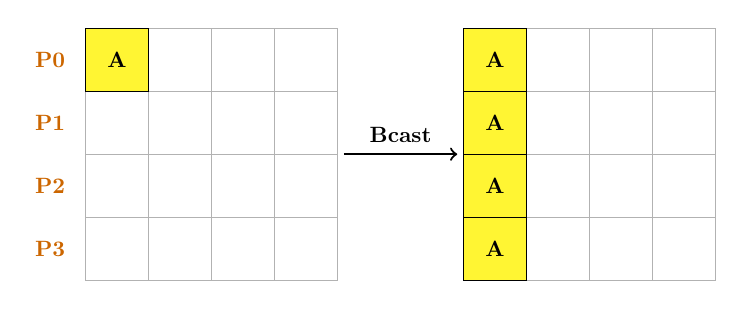
\begin{tikzpicture}[scale=0.8, every node/.style={scale=0.8}]
        %! --- Bcast ---
        % Process labels (left)
        \foreach \i/\p in {0/P0,1/P1,2/P2,3/P3} {
            \node[anchor=east] at (-0.2,3.5-\i) {\textcolor{orange!80!black}{\textbf{\p}}};
        }
        % Bcast left matrix
        \foreach \i in {0,...,3} {
            \foreach \j in {0,...,3} {
                \draw[gray!60] (0+\j,3-\i) rectangle (1+\j,4-\i);
            }
        }
        \node[fill=yellow!80,draw,minimum width=1cm,minimum height=1cm] at (0.5,3.5) {\textbf{A}};
        % Bcast right matrix
        \foreach \i in {0,...,3} {
            \foreach \j in {0,...,3} {
                \draw[gray!60] (6+\j,3-\i) rectangle (7+\j,4-\i);
            }
            \node[fill=yellow!80,draw,minimum width=1cm,minimum height=1cm] at (6.5,3.5-\i) {\textbf{A}};
        }
        % Bcast arrow and label
        \draw[->,thick] (4.1,2) -- (5.9,2);
        \node at (5,2.3) {\textbf{Bcast}};
    \end{tikzpicture}
    % \caption{Broadcast}
    \label{fig:bcast}
\end{figure}

\item \textbf{Scatter and Gather:} The \plaintt{MPI\_Scatter} and \plaintt{MPI\_Gather} functions are complementary collective operations that distribute and collect data among processes. \plaintt{MPI\_Scatter} takes data from a single process (the root) and distributes it among all processes, while \plaintt{MPI\_Gather} does the opposite - it collects data from all processes and combines it at the root.

\begin{figure}[H]
    \centering
    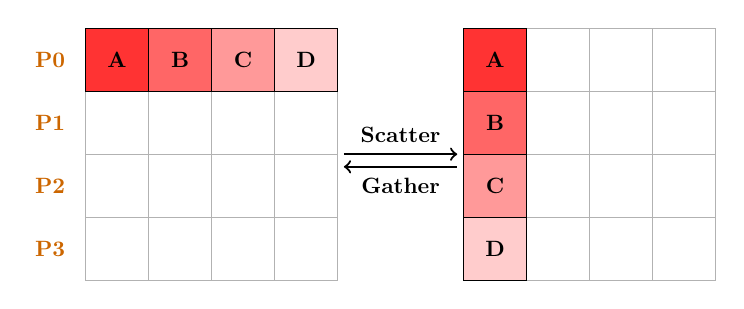
\begin{tikzpicture}[scale=0.8, every node/.style={scale=0.8}]
        %! --- Scatter / Gather ---
        % Process labels (left)
        \foreach \i/\p in {0/P0,1/P1,2/P2,3/P3} {
            \node[anchor=east] at (-0.2,3.5-\i) {\textcolor{orange!80!black}{\textbf{\p}}};
        }
        % Scatter left matrix
        \foreach \i in {0,...,3} {
            \foreach \j in {0,...,3} {
                \draw[gray!60] (0+\j,3-\i) rectangle (1+\j,4-\i);
            }
        }
        \node[fill=red!80,draw,minimum width=1cm,minimum height=1cm] at (0.5,3.5) {\textbf{A}};
        \node[fill=red!60,draw,minimum width=1cm,minimum height=1cm] at (1.5,3.5) {\textbf{B}};
        \node[fill=red!40,draw,minimum width=1cm,minimum height=1cm] at (2.5,3.5) {\textbf{C}};
        \node[fill=red!20,draw,minimum width=1cm,minimum height=1cm] at (3.5,3.5) {\textbf{D}};

        % Scatter right matrix
        \foreach \i in {0,...,3} {
            \foreach \j in {0,...,3} {
                \draw[gray!60] (6+\j,3-\i) rectangle (7+\j,4-\i);
            }
        }
        \node[fill=red!80,draw,minimum width=1cm,minimum height=1cm] at (6.5,3.5) {\textbf{A}};
        \node[fill=red!60,draw,minimum width=1cm,minimum height=1cm] at (6.5,2.5) {\textbf{B}};
        \node[fill=red!40,draw,minimum width=1cm,minimum height=1cm] at (6.5,1.5) {\textbf{C}};
        \node[fill=red!20,draw,minimum width=1cm,minimum height=1cm] at (6.5,0.5) {\textbf{D}};
        % Scatter arrow and label
        \draw[->,thick] (4.1,2) -- (5.9,2);
        \node at (5,2.3) {\textbf{Scatter}};
        
        % Gather arrow and label
        \draw[<-,thick] (4.1,1.8) -- (5.9,1.8);
        \node at (5,1.5) {\textbf{Gather}};
    \end{tikzpicture}
    % \caption{Scatter and Gather}
    \label{fig:scatter-gather}
\end{figure}

\item \textbf{Allgather:} The \plaintt{MPI\_Allgather} function is a collective operation that allows all processes in a communicator to exchange data with all other processes. It collects data from all processes and combines it at the root.

\begin{figure}[H]
    \centering
    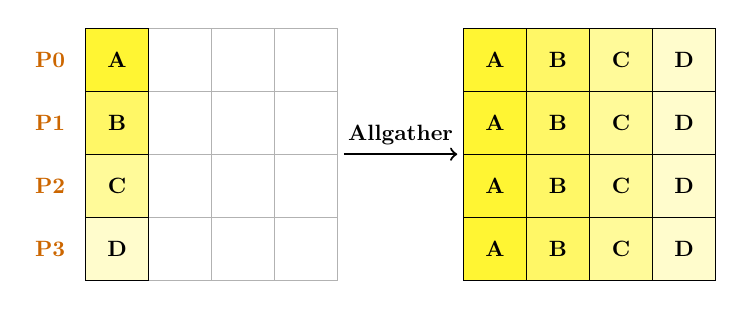
\begin{tikzpicture}[scale=0.8, every node/.style={scale=0.8}]
        % Process labels (left)
        \foreach \i/\p in {0/P0,1/P1,2/P2,3/P3} {
            \node[anchor=east] at (-0.2,3.5-\i) {\textcolor{orange!80!black}{\textbf{\p}}};
        }
        % Allgather left matrix
        \foreach \i in {0,...,3} {
            \foreach \j in {0,...,3} {
                \draw[gray!60] (0+\j,3-\i) rectangle (1+\j,4-\i);
            }
        }
        \node[fill=yellow!80,draw,minimum width=1cm,minimum height=1cm] at (0.5,3.5) {\textbf{A}};
        \node[fill=yellow!60,draw,minimum width=1cm,minimum height=1cm] at (0.5,2.5) {\textbf{B}};
        \node[fill=yellow!40,draw,minimum width=1cm,minimum height=1cm] at (0.5,1.5) {\textbf{C}};
        \node[fill=yellow!20,draw,minimum width=1cm,minimum height=1cm] at (0.5,0.5) {\textbf{D}};
        % Allgather right matrix
        \foreach \i in {0,...,3} {
            \foreach \j in {0,...,3} {
                \draw[gray!60] (6+\j,3-\i) rectangle (7+\j,4-\i);
            }
        }
        \foreach \j in {0,...,3} {
            \node[fill=yellow!80,draw,minimum width=1cm,minimum height=1cm] at (6.5,3.5-\j) {\textbf{A}};
            \node[fill=yellow!60,draw,minimum width=1cm,minimum height=1cm] at (7.5,3.5-\j) {\textbf{B}};
            \node[fill=yellow!40,draw,minimum width=1cm,minimum height=1cm] at (8.5,3.5-\j) {\textbf{C}};
            \node[fill=yellow!20,draw,minimum width=1cm,minimum height=1cm] at (9.5,3.5-\j) {\textbf{D}};
        }
        % Allgather arrow and label
        \draw[->,thick] (4.1,2) -- (5.9,2);
        \node at (5,2.3) {\textbf{Allgather}};
    \end{tikzpicture}
    % \caption{Allgather}
    \label{fig:allgather}
\end{figure}

\item \textbf{Alltoall:} The \plaintt{MPI\_Alltoall} function is a collective operation that allows all processes in a communicator to exchange data with every other process. Each process sends data to every other process, and each process receives data from every other process.

\begin{figure}[H]
    \centering
    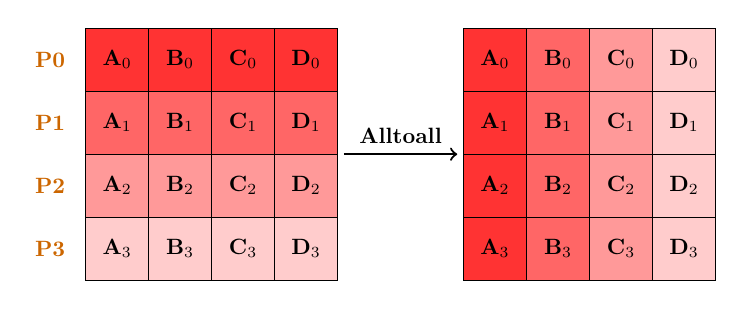
\begin{tikzpicture}[scale=0.8, every node/.style={scale=0.8}]
        % Process labels (left)
        \foreach \i/\p in {0/P0,1/P1,2/P2,3/P3} {
            \node[anchor=east] at (-0.2,3.5-\i) {\textcolor{orange!80!black}{\textbf{\p}}};
        }
        % Alltoall left matrix
        \foreach \i in {0,...,3} {
            \foreach \j in {0,...,3} {
                \draw[gray!60] (\j,3-\i) rectangle (1+\j,4-\i);
            }
        }
        % Fill left matrix
        \foreach \j/\lbl/\col in {0/A,1/B,2/C,3/D} {
            \node[fill=red!80,draw,minimum width=1cm,minimum height=1cm] at (0.5+\j,3.5) {\textbf{\lbl$_0$}};
            \node[fill=red!60,draw,minimum width=1cm,minimum height=1cm] at (0.5+\j,2.5) {\textbf{\lbl$_1$}};
            \node[fill=red!40,draw,minimum width=1cm,minimum height=1cm] at (0.5+\j,1.5) {\textbf{\lbl$_2$}};
            \node[fill=red!20,draw,minimum width=1cm,minimum height=1cm] at (0.5+\j,0.5) {\textbf{\lbl$_3$}};
        }
        % Alltoall right matrix
        \foreach \i in {0,...,3} {
            \foreach \j in {0,...,3} {
                \draw[gray!60] (6+\j,3-\i) rectangle (7+\j,4-\i);
            }
        }
        % Fill right matrix (transpose)
        \foreach \i/\lbl/\col in {0/A,1/B,2/C,3/D} {
            \node[fill=red!80,draw,minimum width=1cm,minimum height=1cm] at (6.5,3.5-\i) {\textbf{A$_\i$}};
            \node[fill=red!60,draw,minimum width=1cm,minimum height=1cm] at (7.5,3.5-\i) {\textbf{B$_\i$}};
            \node[fill=red!40,draw,minimum width=1cm,minimum height=1cm] at (8.5,3.5-\i) {\textbf{C$_\i$}};
            \node[fill=red!20,draw,minimum width=1cm,minimum height=1cm] at (9.5,3.5-\i) {\textbf{D$_\i$}};
        }
        % Alltoall arrow and label
        \draw[->,thick] (4.1,2) -- (5.9,2);
        \node at (5,2.3) {\textbf{Alltoall}};
    \end{tikzpicture}
    % \caption{Alltoall}
    \label{fig:alltoall}
\end{figure}
\end{itemize}

\subsection*{Groups and communicators}

The situation in which a task is preparing data and distributing the work among the other tasks is called \textbf{director/orchestra paradigm}. The final reduce must happen only among the workers, excluding the director task. That would not be a problem, since it would suffice that the director had a zero-valued variable to participate to the reduce. However, this is the case to illustrate how to create new groups and communicators.

When you want to derive a group from an existing communicator, as first you need to "extract" the group of tasks associated with the communicator:
\begin{codeblock}[language=C]
MPI_Group group;
MPI_Comm_group( communicator, &group );
\end{codeblock}
Then, you manipulate the group. For example by selecting/excluding some of the tasks:
\begin{codeblock}[language=C]
MPI_Group_excl( group, n, ranks, &newgroup );
MPI_Group_incl( group, n, ranks, &newgroup );
MPI_Group_range_excl( group, n, ranges, &newgroup );
MPI_Group_range_incl( group, n, ranges, &newgroup );
MPI_Group_union( group1, group2, &newgroup );
\end{codeblock}
Finally, you create a new communicator from the new group:
\begin{codeblock}[language=C]
MPI_Comm newcomm;
MPI_Comm_create( communicator, newgroup, &newcomm );
MPI_Group_free( &group ); /* free the old group */
MPI_Group_free( &newgroup ); /* free the new group */
\end{codeblock}

\begin{observationblock}
    A communicator holds an internal reference to the group, we don't need the groups anymore after the communicator has been created.
\end{observationblock}

Alternatively, it is also possible to operate on the original communicator, subdividing it in two sections:
\begin{codeblock}[language=C]
MPI_Comm new_comm;
MPI_Comm_split( communicator, color, key, &new_comm );
\end{codeblock}
then you'll need to know what are the ranks in the new communicator
\begin{codeblock}[language=C]
MPI_Comm_size( new_comm, &new_size );
MPI_Comm_rank( new_comm, &new_rank );
\end{codeblock}
The root task will get \plaintt{MPI\_INVALID} as \plaintt{Myrank\_new} and \plaintt{new\_comm\_size} and \plaintt{MPI\_COMM\_NULL} as \plaintt{new\_comm}.